\documentclass[10pt,twocolumn]{article}
\usepackage{times}
\usepackage{graphicx}
\usepackage{amssymb}
\usepackage{titling}
\usepackage{url,hyperref}

\begin{document}

\title{Audio Noise Clustering}

\author{Dror Ayalon (dda290)}

\date{%
CUSP-GX-5006 Machine Learning for Cities (NYU)\\
Final Project\\
\rule{\textwidth}{1pt}
}

\posttitle{\par\rule{3in}{0.4pt}\end{center}\vskip 0.5em}
%\postdate{\rule{\textwidth}{1pt}}

\maketitle

\begin{abstract}
  Clustering is a major task in machine learning and many different clustering techniques are available. Very small academical effort was invested in finding the intersection between machine learning algorithms and digital signal processing (DSP) tasks. This research tried to utilize clustering algorithms, in particular spectral clustering and Independent Component Analysis, to reduce noise from speech centric audio recordings. The results were compared with a noise-reduced outcome, which was generated using existing post-production techniques, such as equalizing and frequency band-passes, that were implemented using Python. The noise-reduced audio outcome using machine learning algorithms was not as good as the audio outcome using post-production techniques, but led to some interesting conclusions and ideas for further research. All results could be heard on this url - https://dodiku.github.io/audio\_noise\_clustering/results .
\end{abstract}


\section{Introduction}

Voice interfaces become more common for day-to-day communication. Mobile devices users tend to use these interfaces on-the-go in very noisy environments.
The main goal of this research was to analyze an audio recording and to find the model that could cluster the signal into two groups: "speech" and "noise". Another motivation for this research was to find a computational efficient way to perform this complicated task in real-time applications, without the need for a long and costly deep-learning process.

\begin{figure}[!h]
  \begin{center}
    \includegraphics[width=2.5in]{images/01.png}
  \end{center}

  \caption{The audio recording represented as a time-series (amplitude over time).}
  \label{time-series}
\end{figure}


\section{Methods and Data Sets}

\begin{enumerate}
  \item Audio signal as a dataset - In order to run machine learning algorithms on the audio signal, there was a need to convert the digital audio time series (see figure~\ref{time-series}) into a dataset the could be clustered. The audio signal was converted into two types of data structures:
  \begin{enumerate}
      \item Spectrogram - After running a short-time Fourier transform on the audio signal using LibROSA \cite{ref1}, a Python audio analysis package, the signal could be represented as a spectrogram using a a matrix, which provides data about the intensity of each frequency range within a time frame (see figure~\ref{spectrogram}). Each cell on the matrix is a data sample.

      \begin{figure}[!h]
        \begin{center}
          \includegraphics[width=2.5in]{images/02.png}
        \end{center}

        \caption{The audio recording represented as a spectrogram (frequency bins over time).}
        \label{spectrogram}
      \end{figure}

      \item 3D table - Another way to represent the audio signal data is using a 3-dimensional table (see figure~\ref{table}), where each row is a single sample of the data. The data on each and every sample is structured as follows:
      \begin{enumerate}
      \item Column 1: A numeric value that represents the time-frame number of the sample.
      \item Column 2: A numeric value that represents the the frequency range of the sample.
      \item Column 3: The level of intensity of the sample (the frequency range in the time-frame).

      \begin{figure}[!h]
        \begin{center}
          \includegraphics[width=2.5in]{images/03.png}
        \end{center}

        \caption{The audio recording represented as a 3D table, where each row includes attributes on a specific sample.}
        \label{table}
      \end{figure}

    \end{enumerate}
    Using these 2 different data structures as an input to the spectral clustering algorithm generated different results (more on that on the results section). Another motivation behind the usage of 3D table as a dataset structure was the ability to visualize the data using scatter plots, where each sample is a point on the plot. The visualization allowed a closer and cleared investigation of the clustering results (see example in figure~\ref{clustering-example}).

  \end{enumerate}

  \begin{figure}[!h]
    \begin{center}
      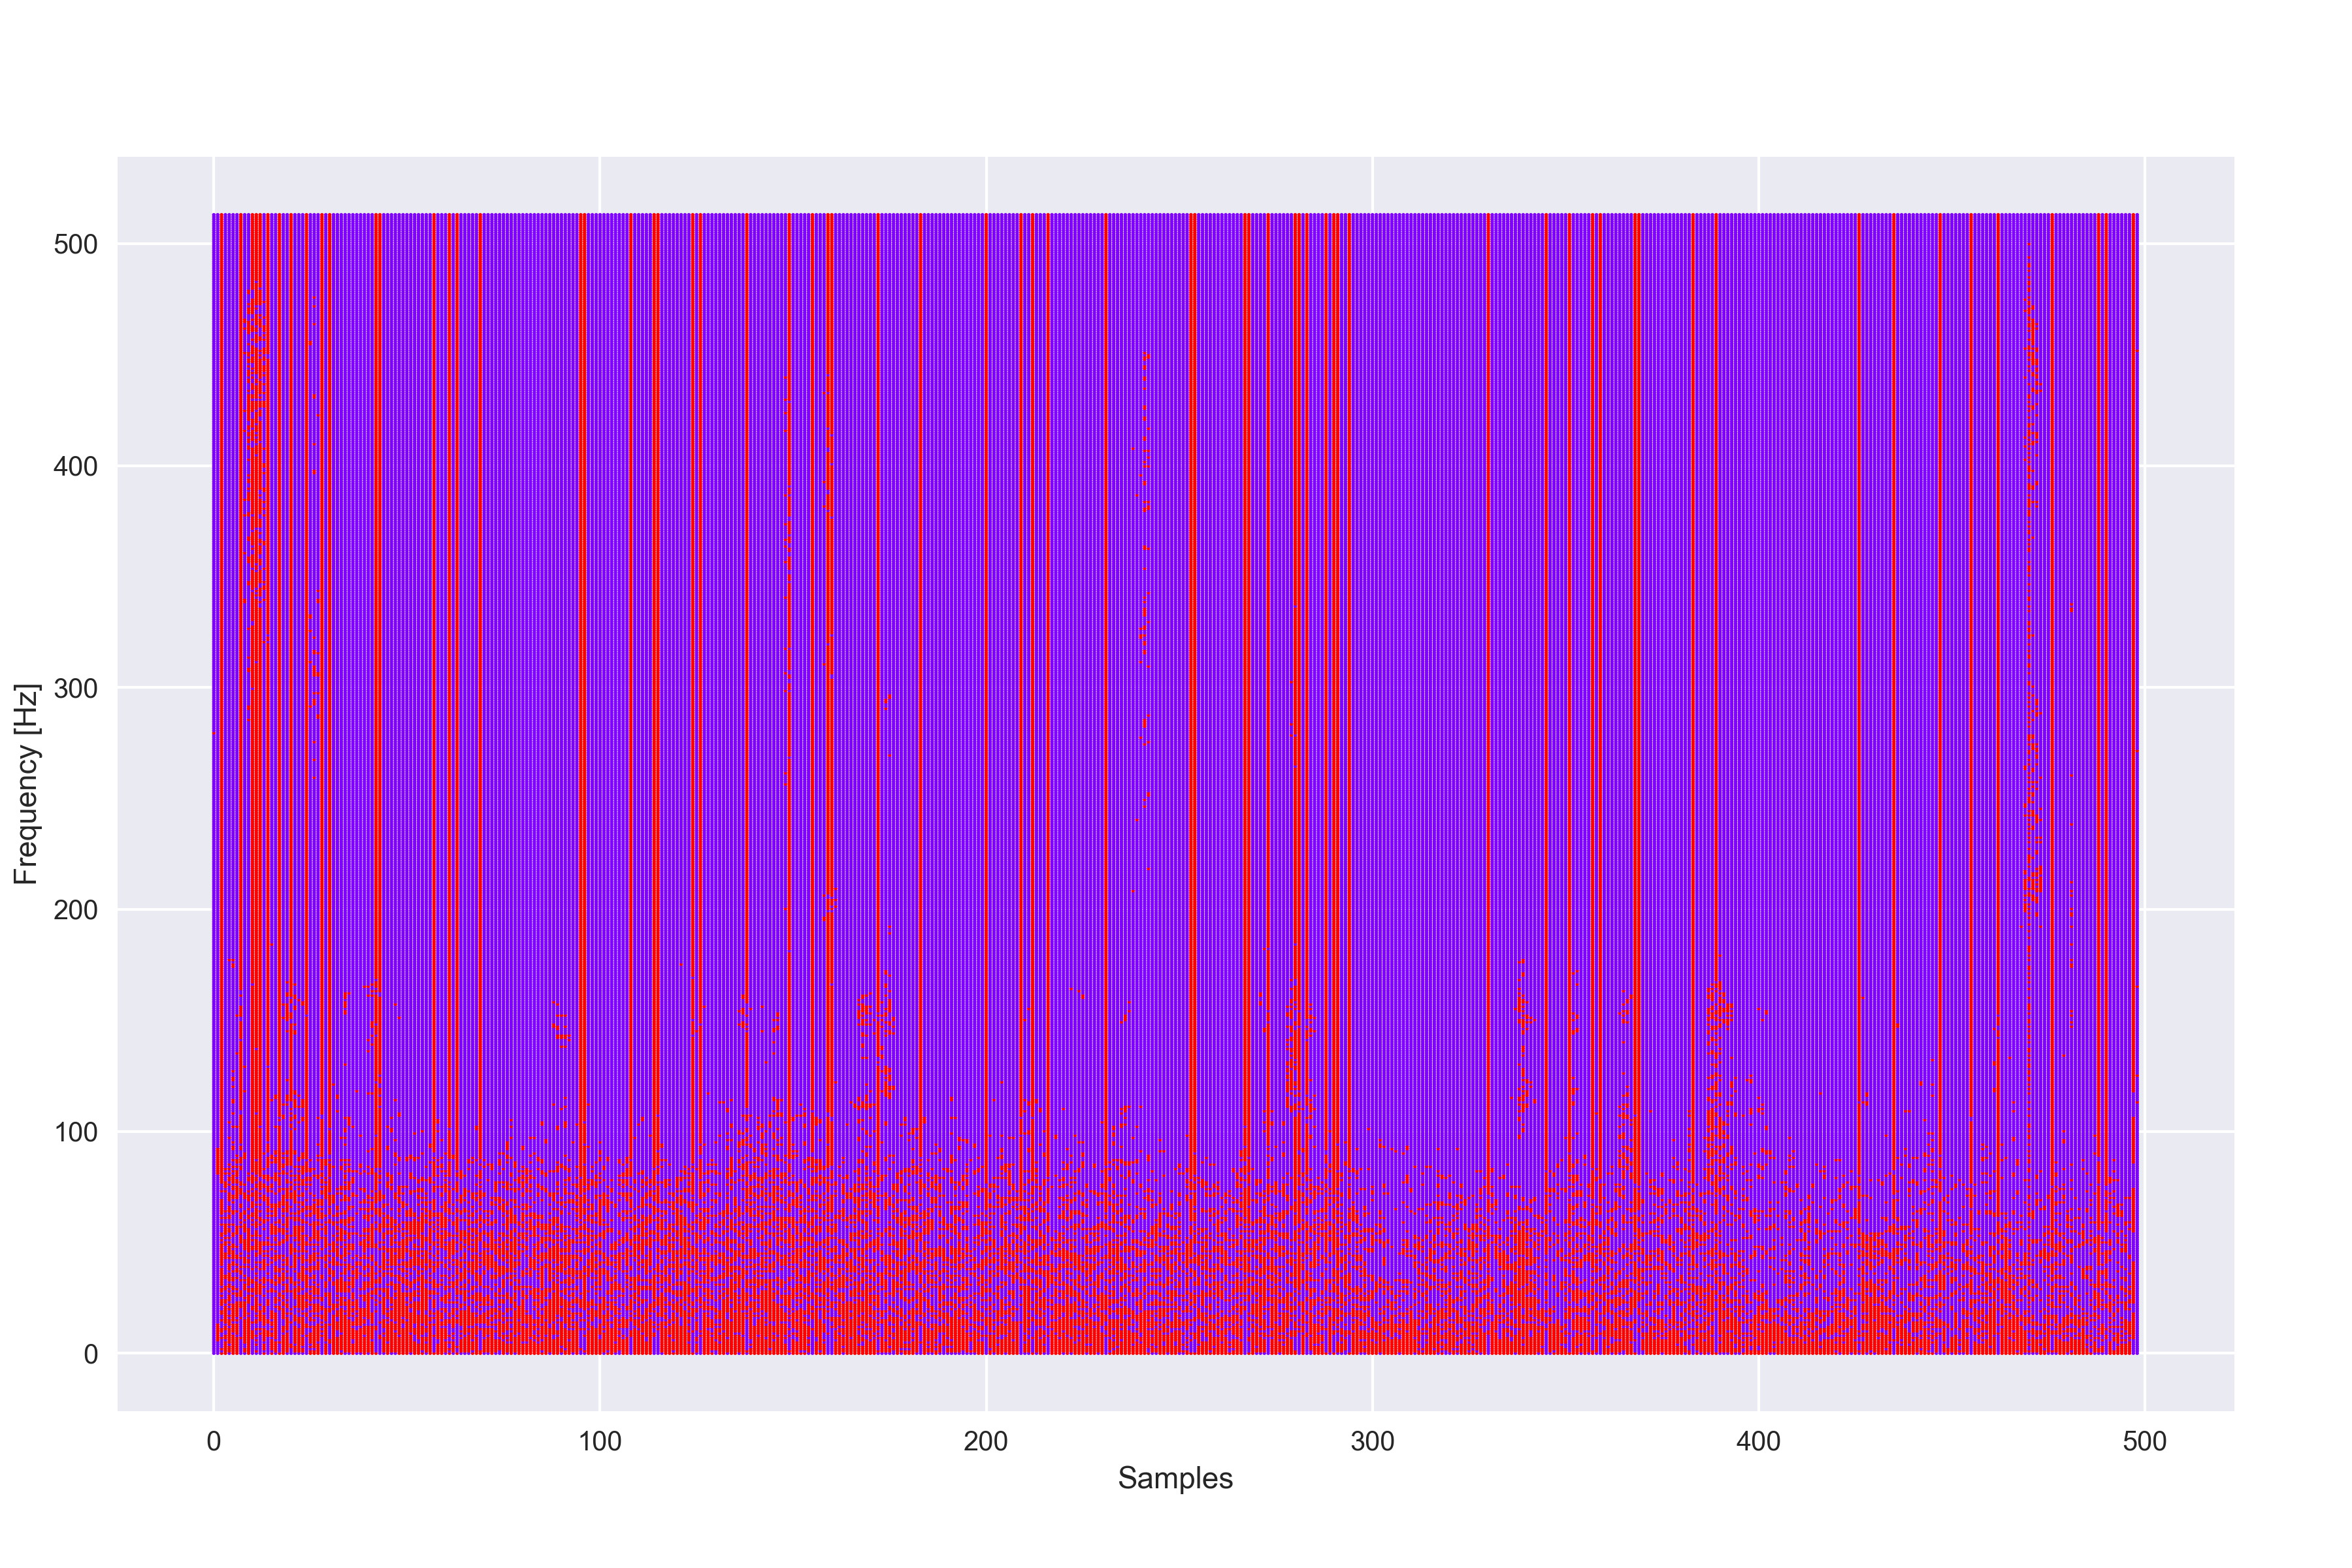
\includegraphics[width=2.5in]{images/04.png}
    \end{center}
    \caption{An example from one of the results of a spectral clustering on a 3D dataset, that represents a spectrogram of an audio signal.}
    \label{clustering-example}
  \end{figure}

  \item The research was done using Python3 and the machine learning Python package scikit-learn (http://scikit-learn.org/). The following scikit-learn algorithms were used to the generate the results for this research:
    \begin{itemize}
      \item Spectral clustering (\texttt{sklearn.cluster.SpectralClustering}) \cite{ref2} - To split noisy frequencies from speech frequencies, a variety of spectral clustering techniques were tested during this research. The largest variation in the outcomes were generated using "rbf" VS. "nearest\_neighbors" as methods to create the affinity matrix, and "discretize" VS. "kmeans" as methods to assign the clustering labels (more about that on the results section).\\
            The spectral clustering algorithm was applied on both structures of the the dataset (spectrogram and 3D table) using 2 strategies:
        \begin{enumerate}
          \item Complete approach: The entire dataset was used as an input for the algorithm.
          \item Column-by-column approach: Applying the spectral clustering algorithm on each and every time frame separately.
        \end{enumerate}
        Each of these strategies generated very different results (more about that on the results section).
      \item Independent Component Analysis (\texttt{sklearn.decomposition.FastICA}) \cite{ref4} \cite{ref3} - An ICA algorithm was used as another method to split noise from speech (see figure~\ref{ica}). Since the ICA algorithm receives 2 inputs (in our case, audio signals) and generates 2 outputs based on the estimated source of the signal (speech and background noise), all possible combinations of the following audio signals were used as inputs:
        \begin{itemize}
          \item The original recording
          \item A noise reduced version of the original recording using post-production techniques
          \item Audio signal that was clustered as "noise" using the spectral clustering algorithm with the complete spectrogram matrix as a dataset
          \item Audio signal that was clustered as "speech" using the spectral clustering algorithm with the complete spectrogram matrix as a dataset
          \item Audio signal that was clustered as "noise" using the spectral clustering algorithm with the complete 3D table as a dataset
          \item Audio signal that was clustered as "speech" using the spectral clustering algorithm with the complete 3D table as a dataset
          \item Audio signal that was clustered as "noise" using the spectral clustering algorithm in a column-by-column approach on the complete spectrogram matrix as a dataset
          \item Audio signal that was clustered as "speech" using the spectral clustering algorithm in a column-by-column approach on the complete spectrogram matrix as a dataset
          \item Audio signal that was clustered as "noise" using the spectral clustering algorithm in a column-by-column approach on the complete 3D table as a dataset
          \item Audio signal that was clustered as "speech" using the spectral clustering algorithm in a column-by-column approach on the complete 3D table as a dataset
        \end{itemize}
        It is important to mention that using different parameters on the spectral clustering algorithm, each of the methods specified above generated different clusters, and therefore, different signals. All these different outcomes where used as an input for the ICA algorithm. The best results are shown on the results section.
        \begin{figure}[!h]
          \begin{center}
            \includegraphics[width=3.5in]{images/05.png}
          \end{center}
          \caption{The process of convolving two audio signal, and splitting them again, based on their estimated sources, using ICA.}
          \label{ica}
        \end{figure}
    \end{itemize}

  \item Data reduction process - To reduce the computation time, audio recordings were sampled in a regular sampling-rate and a low-resolution sampling-rate. The algorithmic procedures were done on the low-resolution datasets. Then, the low-resolution dataset was stretched to the size of the regular-resolution dataset (see figure~\ref{res}). The clustering results, which where generated on the the low-res dataset, were applied on the stretched regular sized dataset. This method enabled reasonable runtimes for the clustering procedures, and the ability to generate outcome wave files (which can only be generated using the high-res sampling dataset) that were used to evaluate the final results of each run.
  \begin{figure}[!h]
    \begin{center}
      \includegraphics[width=2.5in]{images/06.png}
    \end{center}
    \caption{The process of stretching a low-res dataset (audio signal spectrogram) to the size of the regular dataset, without loosing the main features and structure of the dataset.}
    \label{res}
  \end{figure}

  \item To summarize, the work process for this research was as follows:
    \begin{enumerate}
      \item Load audio file
      \item Sample the audio file, using a low-res sample-rate and a regular-res sample-rate, to generate audio time series.
      \item Convert the audio time series to a spectrogram of amplitudes (matrix, bins * frames) using a Short-time Fourier transform.
      \item (optional) Change the structure of the data to improve clustering results
      \item Cluster the data using the spectral clustering algorithm
      \item Stretch the low-res dataset to the size of the regular-size dataset
      \item Apply the clustering results on the stretched dataset
      \item Remove (or reduce) the samples that were clustered as noise
      \item Run Inverse short-time Fourier transform to convert the spectrogram back to an audio time series
      \item Write a file using the new time series array
Compare results sonically
    \end{enumerate}

\end{enumerate}

\section{Results}

\begin{enumerate}
  \item All outcomes could be heard on the following url - https://dodiku.github.io/audio\_noise\_clustering/results/

  \begin{figure}[!h]
    \begin{center}
      \includegraphics[width=3in]{images/07.png}
    \end{center}
    \caption{LEFT: Clustering results for the complete spectrogram as a dataset. RIGHT: Applying the clustering reults on the speech recording.}
    \label{07}
  \end{figure}

  \item A very "naive" result was generated using the spectrogram (matrix) as dataset, and clustering the data using the "complete approach", while "nearest\_neighbors" was set to create the affinity matrix (adjacency matrix) and "arpack" as the eigen solver (see figure~\ref{07} or listen to the best results under "spectral clustering 01 - Spectrogram" on the results webpage).
  \\In terms of computation time, this result was generated relatively quickly (Runtime = 4.4s for a 10s recording), but was not satisfying enough sonically.

\item Very interesting results were generated using the spectrogram (matrix) as dataset in a "column-by-column" approach, and while "rbf" was set as the method to create the affinity matrix. The clustering algorithm was able to pick-up the dominant parts of the recording (see figure~\ref{09}), but the outcomes have many artifacts and the isolated speech is not clear enough (listen to the best results under "spectral clustering 02 - Column-by-Column" on the results webpage).
\\The main drawback of this result was the long run-time (24.2s-26.9s on a low-res dataset, ~1:30h on a regular-res dataset for a 10s recording).

\begin{figure}[!h]
  \begin{center}
    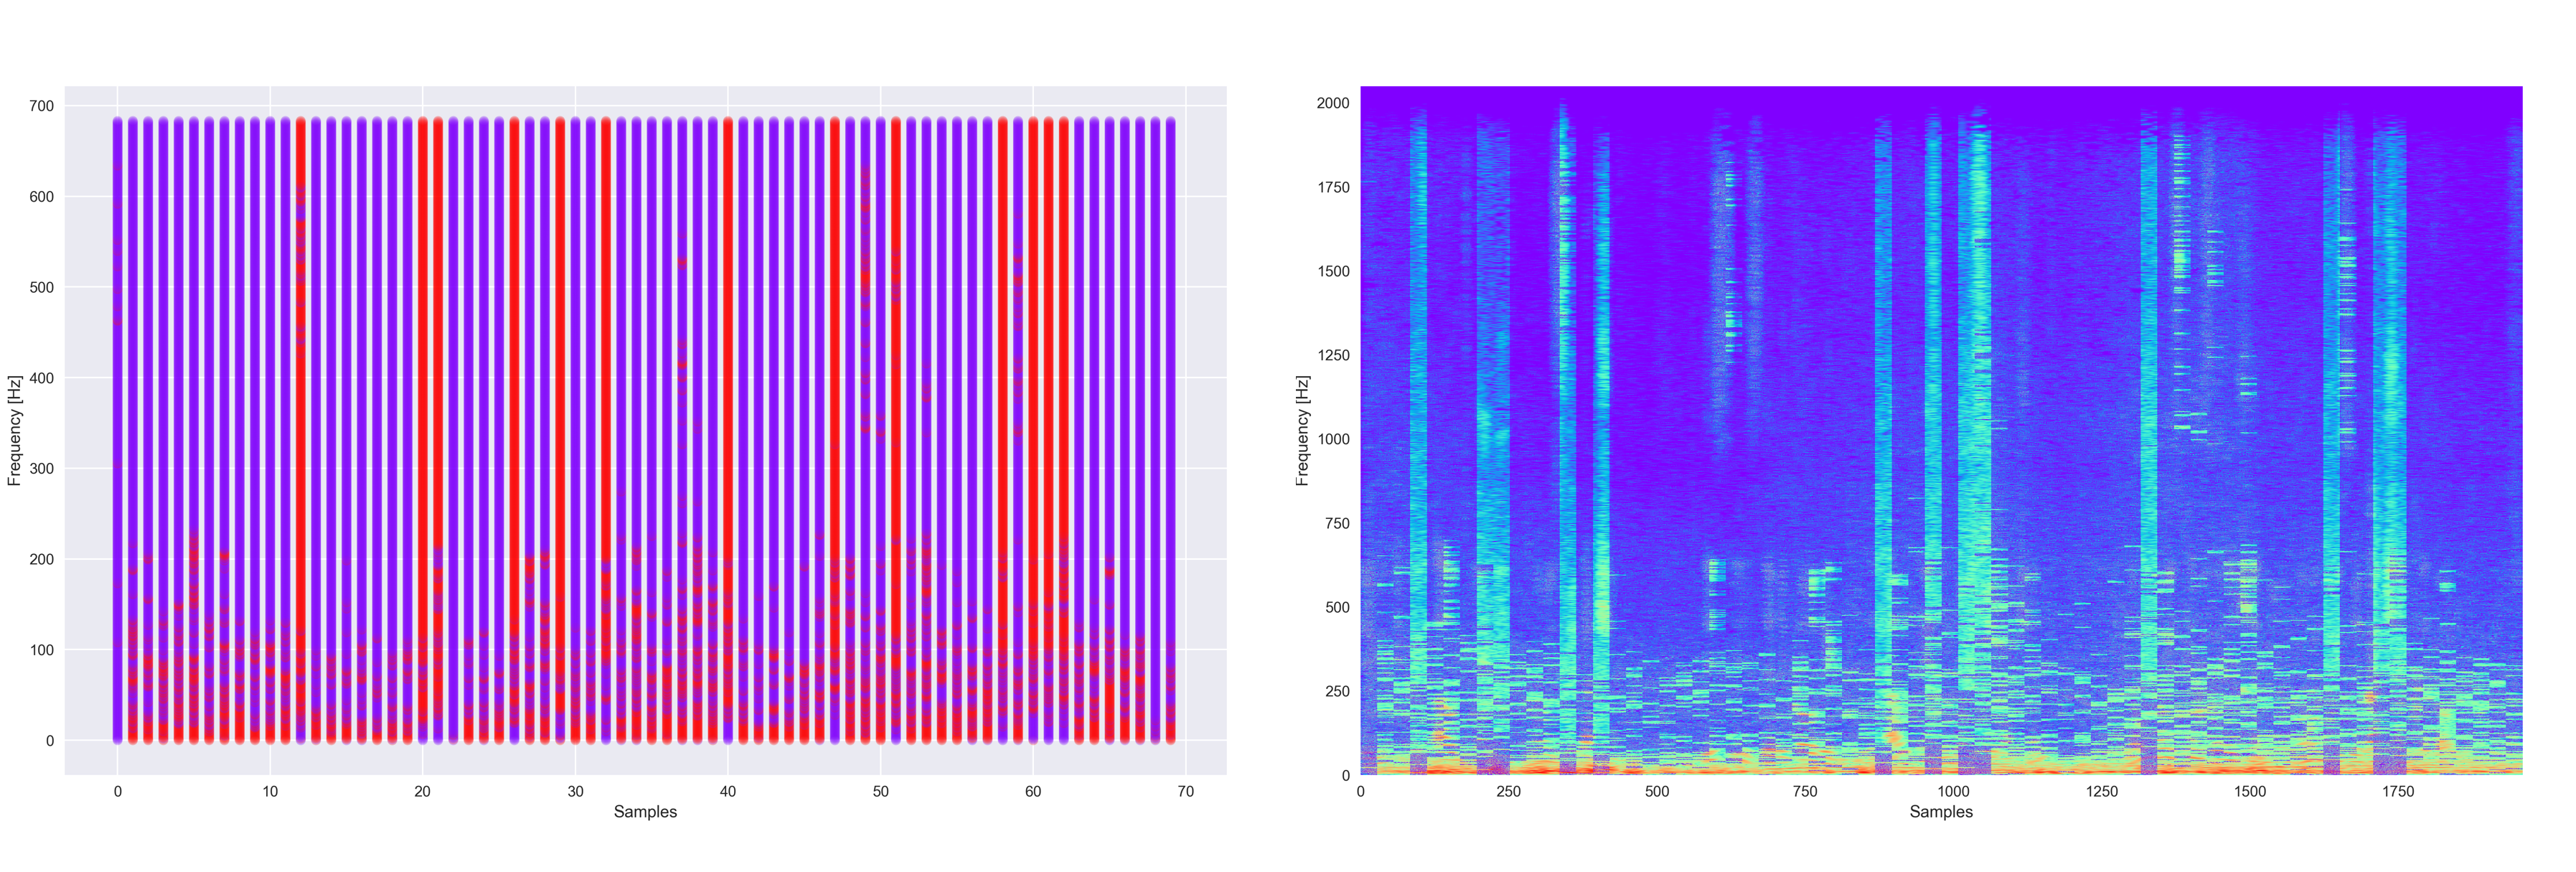
\includegraphics[width=3in]{images/09.png}
  \end{center}
  \caption{LEFT: Clustering results for the complete spectrogram as a dataset in a "column-by-column" approach. RIGHT: Applying the clustering reults on the speech recording.}
  \label{09}
\end{figure}

\item The best result from the spectral algorithm alone, was generated when the input was the 3D table as dataset using a "column-by-column" approach (see figure~\ref{10}, or listen under "spectral clustering 04 - Column-by-Column from a 3D table" on the results webpage).
\\This result was the best sonically, but was very heavy in terms of computation time (Runtime = ~34.4s for low-res dataset, and ~2.5h for a regular-res dataset for a 10s recording).

\item Two very interesting results were generated using the ICA algorithm. On one of these cases, the inputs to the ICA algorithm were:
\begin{enumerate}
  \item The speech cluster outcome from spectral clustering using column-by-column approach on a 3D table.
  \item The speech cluster outcome from spectral clustering using complete spectrogram.
\end{enumerate}
On the other case, the inputs to the ICA algorithm were:
\begin{enumerate}
  \item The speech cluster outcome from spectral clustering using column-by-column approach on a 3D table.
  \item ICA result using:
  \begin{enumerate}
    \item The speech cluster outcome from spectral clustering using column-by-column approach on a 3D table and "kmeans" as to assign the clustering labels.
    \item A noise reduced version of the original recording using post-production techniques.
  \end{enumerate}
\end{enumerate}
The last described result is considered to be the best result that was found on this research (listen to these results under "ICA: Independent component analysis" on the results webpage).

\end{enumerate}

\begin{figure}[!h]
  \begin{center}
    \includegraphics[width=3in]{images/10.png}
  \end{center}
  \caption{LEFT: Clustering results for the 3D table as a dataset in a "column-by-column" approach. RIGHT: Applying the clustering reults on the speech recording.}
  \label{10}
\end{figure}

\section{Conclusions}
\begin{enumerate}
\item Since human speech varies between a large range of frequencies, that in most cases overlap with background noise frequencies, it is very hard (maybe impossible) to cluster away noise.
\item The tested clustering technique could not produce better results than existing production techniques.
\item The data reduction and stretch technique was very successful in reducing the computation time of the clustering process, while not harming the outcomes of the process.
\item Using results from spectral clustering using the "complete approach" and the "column-by-column" approach as inputs to and ICA algorithm could produce promising results.
\item This research did not show promising reults using the noise frequencies, as clustered by the spectral clustering algorithm. This might be due to the similarity of the noise on the "speech" cluseter and on the "noise" cluster.
\item Using the entire spectrogram as an input to the spectral algorithm tend to generate "naive" clusters. This behaviour makes sense since the distance between two frequency bins on different time frame (different column) is an important factor that effects algorithm"s affinity matrix.
\end{enumerate}

\bibliographystyle{abbrv}
\bibliography{refs}
\end{document}
